\documentclass[a4paper,12pt]{extarticle}
\usepackage[margin=1.5cm]{geometry}
\usepackage{amsmath, amssymb}
\usepackage{array}
\usepackage{multicol}
\usepackage{helvet}
\usepackage{multirow}
\usepackage{graphicx}


\usepackage{amsmath, amsfonts, amssymb}
\usepackage{xcolor}
\usepackage{tikz}
\usepackage{enumitem}

\definecolor{numcolor}{RGB}{180, 0, 0}

\pagestyle{empty}


\renewcommand{\baselinestretch}{2}
\renewcommand{\familydefault}{\sfdefault}

\begin{document}

    \begin{tabular}{| c | c | c | c |}
        \hline
        & MATEMÁTICAS  &Fecha:$\hspace{2.5cm}$   & Calificación \\
        \hline 

        \multirow{2}{*}{
\includegraphics[scale=0.15]{../../img-Logos/IesSierraCarrascoy.png}} & Nombre y apellidos \hspace{120pt} & Ex. 4º ESO   & \\ 
        &&UD2& \\ 
        \hline
    \end{tabular}
    
    \begin{tabular}{| l | }
        \hline
        NOTAS: \\ 
            1. El examen tiene que ser limpio, ordenado y sin faltas de ortografía. \\
            
            2. El examen ha de realizarse en bolígrafo negro o azul, evitando tachones en la medida \\
            de lo posible. \\ 
            
            3. Deben aparecer todas las operaciones NO vale con indicar solo el resultado.\\
            
            4. Los problemas deben contener: Datos, planteamiento y resolución, respondiendo a lo \\
            que se pregunte, NO vale con indicar un número como solución del problema.\\

            5. Persona que se vea copiando o hablando con un compañero tiene un cero en el examen\\

            6. \textbf{NO} está permitido el uso de la calculadora. \\ 
        \hline
    \end{tabular}

    \begin{enumerate}
        \item \textbf{Opera y simplifica:}
            \[
                \frac{(x - 2)(x + 1)}{3} - \frac{(3x - 1)^2}{8} + \frac{(2x - 3)(2x + 3)}{12} =
            \]
        \item \textbf{Halla el cociente y el resto de la división:}
            \[
                3x^4 - 5x^3 + 4x^2 - 1 \;\Big|\!\underline{\;x^2 + 2\;}
            \]
        \item \textbf{Descompón en factores los siguientes polinomios:}
            \begin{enumerate}[label=\alph*), itemsep=0.5em]
                \item $x^4 - 12x^3 + 36x^2$
                \item $2x^4 + 5x^2 - 4x - 3$
            \end{enumerate}
        \item \textbf{Calcula el valor del parámetro {\color{numcolor}$m$} para que el polinomio $P(x) = 7x^3 - mx^2 + 3x - 2$, sea divisible por $x + 1$.}
        \item \textbf{Simplifica las siguientes fracciones algebraicas:}
            \begin{enumerate}[label=\alph*), itemsep=0.8em]
                \item $\dfrac{x^3 - 4x}{x^3 + x^2 - 2x}$
                \item $\dfrac{x^2 + 2x - 3}{x^3 + 6x^2 + 5x - 12}$
            \end{enumerate}
        \item \textbf{Efectúa y simplifica cuando sea posible:}
            \begin{enumerate}[label=\alph*), itemsep=0.8em]
                \item $\dfrac{2x^2}{x - 3} : \dfrac{8}{x^3 - 3x^2}$
                \item $\dfrac{x^2 - 6}{(x - 2)^2} - \dfrac{x - 3}{x - 2}$
            \end{enumerate}
        \item \textbf{En un triángulo rectángulo, un cateto mide $14\text{ cm}$. Escribe el perímetro y el área del triángulo en función de su hipotenusa $x$.}
        \item \textbf{En una parcela de lados $x$ e $y$ se construye una casa, en la zona que se indica en la figura.}
            \begin{center}
                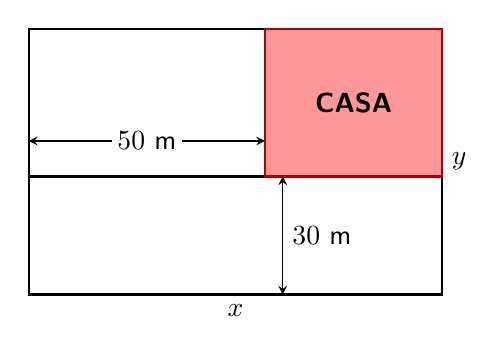
\begin{tikzpicture}[scale=0.075]
                % Parcela total
                \draw[thick] (0,0) rectangle (70,45);
                
                % Zona no edificada / delimitaciones (líneas continuas de referencia)
                \draw[thick] (0,20) -- (40,20) -- (40,45);
                
                % Casa (relleno y borde)
                \fill[red!40] (40,20) rectangle (70,45);
                \draw[thick, red!70!black] (40,20) rectangle (70,45);
                \node at (55, 32.5) {\textbf{CASA}};
                
                % Cotas y medidas
                % 50 m (arriba a la izquierda)
                \draw[<->, >=stealth] (0,26) -- (40,26);
                \node[fill=white, inner sep=2pt] at (20,26) {$50\text{ m}$};
                
                % 30 m (abajo en el interior)
                \draw[<->, >=stealth] (43,0) -- (43,20);
                \node[right] at (43,10) {$30\text{ m}$};
                
                % Etiqueta x abajo
                \node[below] at (35,0) {$x$};
                
                % Etiqueta y a la derecha
                \node[right] at (70,22.5) {$y$};
                \end{tikzpicture}
            \end{center}
    Expresa en función de $x$ e $y$ el área de la zona no edificada.
    \end{enumerate}

\end{document}